\documentclass[9pt,twocolumn,twoside]{osajnl}

\usepackage{multirow}

\journal{jocn} 

% See template introduction for guidance on setting shortarticle option
\setboolean{shortarticle}{false}
% true = letter / tutorial
% false = research / review article
% (depending on journal).

\title{Simulazione di un filtro digitale per la rilevazione di segnali neurali \emph{ }}

\author[1]{Alfredo Guarnieri}
% \author[2,*]{Author Two}
% \author[1]{Author Three}

% \affil[1]{Publications Department, The Optical Society (OSA), 2010 Massachusetts Avenue NW, Washington D.C., 20036, USA}
% \affil[2]{School of Science, University of Technology, 2000 J St. NW, Washington DC, 20036, USA}
% \affil[3]{School of Optics, University of Technology, 2000 J St. NW, Washington DC, 20036, USA}

% \affil[*]{Corresponding author: email@my-email.com}

%% To be edited by editor
% \dates{Compiled \today}

%\ociscodes{(140.3490) Lasers, distributed feedback; (060.2420) Fibers, polarization-maintaining;(060.3735) Fiber Bragg gratings.}

%% To be edited by editor
% \doi{\url{http://dx.doi.org/10.1364/XX.XX.XXXXXX}}

\begin{abstract}
Le proprietà spettrali di segnali rumorosi di impulsi in tensione caratterizzati da spaziatura e ritardo temporale irregolari, sono utilizzate in questo lavoro con l'intento di simulare un segnale di natura biologica e verificare le capacità predittive di alcuni test di soglia ampiamente utilizzati per la rilevazione di segnali provenienti da popolazioni di neuroni con tecnologia $MEA$, \cite{Lambacher2011}, \cite{Vallicelli2017}. 

L'analisi è condotta parallelamente sotto il profilo spaziale e temporale analizzando la distribuzione congiunta di, (1) una metrica spettrale per la distanza del segnale filtrato da quello originale e (2) un indice di precisione della rilevazione nel tempo degli impulsi.

Si conclude che i test di soglia in tensione a media semplice conducono a risultati più precisi in merito alla rilevazione del tempo degli impulsi. In particolare, rispetto ai test in potenza hanno percentuali di impulsi rilevati sul totale degli impulsi emessi maggiori. Tale proprietà sono verificate per un ampio spettro di $SNR$ e su diversi tipi di impulso. Si conclude che i test a media semplice, facendo leva sull'elevata frequenza di campionamento spazio-temporale della tecnologia utilizzata, consentono di ridurre la rumorosità del segnale mediando segnali da diversi pixel e sono molto precisi sia con riguardo alla rilevazione dello spettro quanto alla previsione dell'esatto momento di emissione dell'impulso. Mostrano inoltre percentuali di corretta rilevazione superiori.
\end{abstract}

% \setboolean{displaycopyright}{true}

\begin{document}

\maketitle



\section{Introduzione}

Nei contesti sperimentali di rilevazione di segnali neurali con tecnologia $MEA$ un segnale fortemente rumoroso nasconde degli impulsi in tensione di forma non nota che si manifestano in tempi non noti, con frequenza media
({\it mean spike rate}) dell'ordine di qualche $kHz$. Le capacità discriminanti di alcuni algoritmi di rilevazione del segnale proposti in letteratura
\cite{Vallicelli2017}, \cite{Lambacher2011} vengono qui confrontati su un segnale di prova.

La simulazione introduce tre tipi di irregolarità suggerite sia dal contesto sperimentale di rilevazione del segnale, che dalla sua natura biologica: (1) rumore termico additivo; (2) intervalli di tempo casuali tra due impulsi successivi; (3) ritardo di fase di campionamento dell'impulso casuale.

Le variabili di simulazione riguardano le seguenti proprietà: (1) la distribuzione di probabilità dei tempi d'attesa tra due impulsi; (2) la forma degli impulsi; (3) lo spike rate medio; (4) SNR. Con riguardo alla prima, analisi preliminari evidenziano che l'emersione dei picchi alla frequenza dello spike rate medio avviene solo quando la deviazione standard della distribuzione dei tempi d'attesa è sufficientemente bassa, è necessario quindi modellare tale distribuzione con almeno due parametri distinti, uno per la media e uno per la varianza. Sono state perciò scartate le più semplici distribuzioni di probabilità come quella rettangolare e quella del decadimento esponenziale\footnote{Note nella letteratura statistica rispettivamente come uniforme ed esponenziale negativa}. La varianza di tali distribuzioni è infatti funzionalmente dipendente dalla media e per la presente applicazione, troppo elevata. La distribuzione utilizzata è invece la distribuzione gamma, controllata da due parametri, uno di forma, detto $\lambda$ e uno di scala, detto $\beta$. La distribuzione gamma è la più semplice generalizzazione della distribuzione esponenziale negativa, potendosi ottenere come distribuzione della somma di un numero $\beta$ di variabili casuali esponenziali negative, tutte identicamente distribuite con parametro di media $\lambda$. In funzione di questi parametri lo spike rate medio è $\beta\lambda$ e la varianza $\beta\lambda^{2}$, in questo modo, variando opportunamente i due parametri $\lambda$ e $\beta$, si ottengono tutte le possibili configurazione dei primi due momenti dello spike rate. Con riguardo invece alla forma degli impulsi, l'analisi preliminare ha evidenziato una certa variabilità dei risultati che giustifica l'utilizzo nella simulazione di una varietà di forme funzionali di impulso. Infine, con riguardo allo spike rate medio, i risultati preliminari non hanno dimostrato sufficiente variabilità in un ampio intervallo di frequenze a partire da qualche decina di $Hz$ fino al limite di $10kHz$, oltre il quale impulsi della durata di $1ms$ iniziano a sovrapporsi.

Nel contesto sperimentale di riferimento, l'elevata densità spaziale dei sensori fa sì che un singolo impulso emesso sia rilevato da un numero di circa $7$ pixel contigui. Perciò, i test utilizzati per la rilevazione del segnale fanno anche leva sul profilo spaziale, utilizzando opportune quantità medie tra i 7 pixel. I test presi in considerazione dalla simulazione sono due, il primo proposto in letteratura da \cite{Lambacher2011}, è un test in potenza basato sulla media quadratica del segnale. Il secondo test, più semplice e utilizzato come test di riferimento, si basa su medie aritmetiche. Ognuno dei due test è variato con due diversi filtri in frequenza, applicati preliminarmente, un passa banda e un passa basso, applicati alternativamente per un totale di quattro test.

Le conclusioni della simulazioni si basano sull'accuratezza delle capacità discriminanti dei due algoritmi di sorting. Nella fase preliminare dell'analisi, l'andamento congiunto di due metriche, una afferente al dominio delle frequenze e una al dominio dei tempi, mostra evidenze a favore dei test a media artimentica, evidenza sì corroborata da un coerente andamento delle metriche al variare di tutte le variabili di simulazione, ma non del tutto conclusiva.

Con il fine di approfondire e confermare tali risultanze intermedie, un'ulteriore verifica della capacità discriminante dei due test viene condotta per mezzo di un'analisi di classificazione delle previsioni, riportata in misura media al variare di tutte le variabili di simulazione e con la ripetizione della simulazione su $100$ iterazioni, in modo da ottenere risultati più robusti con riguardo anche alle casualità introdotte. I risultati di simulazione vengono riassunti in quattro categorie: falsi positivi, veri positivi, falsi negativi e veri negativi. Le conclusioni si affidano a due indici di concordanza, l'indice di concordanza di Jaccard e il punteggio $F1$, noti nella letteratura statistica e ampiamente utilizzati per riportare l'accuratezza degli algoritmi di classificazione. Tali indici, sono da intendersi come delle misure di correlazione\footnote{Trattandosi di variabili dicotomiche è corretto parlare di associazione o concordanza}, tra la previsione dei tempi degli impulsi e i tempi effettivi, e sono, per comodità, uniformati a variare tra il valore $0$, che indica assenza di correlazione e $1$, massima dipendenza. 

I valori degli indici per i filtri a media aritmetica risultanti dalla presente simulazione sono sempre sensibilmente superiori a quelli degli algoritmi a media quadratica, indipendentemente dal tipo di filtro in frequenza applicato. Confermando perciò le evidenze grafiche intermedie.

% This  template is designed to assist with creating an article to submit to the \emph{Journal of Optical Communications and Networking}. See the OSA's \href{http://www.opticsinfobase.org/submit/style/}{Style Guide} and \href{http://www.opticsinfobase.org/submit/templates/}{Manuscript Templates} pages for more details.
% 
% If you have a question while using this template on {Overleaf}, please use the help menu (``?'') on the top bar to search for help or ask us a question using our \href{https://www.overleaf.com/contact}{contact form}.



\section{Simulazione}
\label{sec:examples}

La seguente tabella \ref{tab:param} riporta i parametri di simulazione.

\begin{table}[htbp]
\centering
\caption{\bf Parametri di simulazione}
\begin{tabular}{ccc}
\hline
Durata segnale                  & 1s                \\
Spike rate (media)              & 150Hz             \\
Spike rate (errore standard)    & 0.01              \\
Durata spike                    & 1ms               \\
Ampiezza Max 0p                 & 60mV              \\
Potenza media spike             & 1.8$\mu V^{2}s$   \\
Campionamento                   & 9kSamples         \\
Filtro. $\nu_{low}$             & 0.02 kHz          \\
Filtro. $\nu_{high}$            & 2.5 kHz           \\
Filtro. Tipo e Ordine           & Butterw. $2\textdegree$ \\
Pixels nel cluster              & 7                 \\
\hline
\end{tabular}
\label{tab:param}
\end{table}



\subsection{Impulsi e SNR}

Il segnale di prova è costituito da un treno di impulsi di durata fissa di $D=1ms$ la cui specifica forma funzionale nel tempo è data da una funzione $I(t-t_{j})$, dove $t_{j}$ è il tempo di emissione del $j-$esimo impulso. Con un numero di impulsi $K$, spaziati nel tempo in accordo con il tasso di emissione degli impulsi {\it spike rate}, il segnale in funzione del tempo può perciò essere scritto 
%
\begin{align*}
S(t) & = \sum_{j=1}^{K} I(t - t_{j})Rect(\frac{t-t_{j}}{D}),   \\
\quad t & = 0, ..., T.
\end{align*}
%
Il segnale deterministico $S(t)$ così ottenuto costituisce il segnale di riferimento della simulazione, rispetto al quale, il filtro della seguente versione rumorosa $\tilde{S}(t)$ sarà confrontato.
La versione rumorosa $\tilde{S(t)}$ si ottiene aggiungendo le seguenti irregolarità
%
\begin{align*}
\tilde{S(t)} & = \sum_{j=1}^{K} I(t - \tau_{j})Rect(\frac{t-\tau_{j}-\phi_{j}}{D}) 
 + \epsilon_{t},
 \end{align*}
%
dove $\phi_{j}$ è un ritardo di campionamento casuale distribuito uniformemente nell'intervallo $[0,\frac{1}{\nu_{s}}]$, dove $\nu_{s}$ è il tasso di campionamento. $\tau_{j}$ è il tempo di emissione del $j-$esimo impulso, distribuito secondo la variabile casuale $t_{j-1}+\Gamma(\alpha, \beta)$, dove $t_{j-1}$ è il tempo, noto, di emissione del precedente impulso e $\Gamma(\alpha, \beta)$ è una distribuzione gamma i cui parametri sono fissati in modo da ottenere lo spike rate medio desiderato e il relativo errore standard che garantisca sufficiente regolarità nell'emissione degli impulsi tale da far emergere i picchi spettrali alla frequenza dello spike rate.
%
% \begin{table}[htbp]
% \centering
% \caption{\bf Momenti del tasso di emissione degli impulsi}
% \begin{tabular}{cccc}
% \hline
% Media            & $\beta\lambda$      & $150Hz$   \\
% Varianza         & $\beta\lambda^{2}$  &           \\
% Errore standard  & $\beta$            & $0.01$    \\
% \hline
% \end{tabular}
% \label{tab:momenti}
% \end{table}
%
Infine $\epsilon_{t}$ è un rumore gaussiano di natura termica di media nulla e di varianza determinata in funzione della potenza media del segnale di riferimento e dell'$SNR$ imposto dalla simulazione. La potenza di rumore utilizzata per dato $SNR$ è stata calcolata secondo le seguenti relazioni.
\begin{align*}
P_{thermal noise} \quad [V^2s] &=  P_{impulses signal} 10^{- snr [dB]/10} \\
\sigma^{2}_{\epsilon} &= \frac{ P_{noise} }{ N }
\end{align*}




\subsection{Algoritmi di sorting}

Gli algoritmi di sorting analizzati \ref{alg:arit}, \ref{alg:quad} sono riportati qui di seguito. L'algoritmo \ref{alg:quad} è disegnato per identificare picchi in potenza del segnale e si trova proposto in \cite{Lambacher2011}. L'algoritmo \ref{alg:arit} è un test di riferimento, che esegue una semplice media spaziale del segnale in tensione.
Ognuno dei due algoritmi viene implementato dopo l'applicazione di un filtro in frequenza che può essere, passa basso o passa banda alla frequenze indicate nella tabella \ref{tab:param}, per un totale di $4$ combinazioni.

Si evidenzia qui che per evitare effetti distorsivi sul risultato del confronto tra i due algorimti, l'ultimo passaggio dell'algoritmo \ref{alg:quad} che prevede la media mobile di ordine 3, viene eseguito con un filtro a fase zero, così da evitare che scostamenti di previsione dovuti alla differenza di fase influiscano sulle conclusioni della simulazione, come meglio spiegato nelle conclusioni \ref{conclusioni}.


\begin{algorithm}
\caption{Algoritmo lineare}\label{alg:arit}
\begin{algorithmic}[1]
%\Procedure{Euclid}{$a,b$}\Comment{The g.c.d. of a and b}
\State $s_{j,t}$ \Comment{Segnale al tempo t, pixel j}
\State $f_{j,t}$ \Comment{Filtro passa basso o passa banda}
\State $f_{t}\gets \sum_{1:7}   f_{j,t}/7$ \Comment{Media spaziale}
%\State $f_{t}\gets \sum_{i=1:3} f_{t-i}/3$
% \EndWhile\label{euclidendwhile}
% \State \textbf{return} $b$\Comment{The gcd is b}
% \EndProcedure
\end{algorithmic}
\end{algorithm}


\begin{algorithm}
\caption{Algoritmo quadratico}\label{alg:quad}
\begin{algorithmic}[1]
%\Procedure{Euclid}{$a,b$}\Comment{The g.c.d. of a and b}
\State $s_{j,t}$ \Comment{Segnale al tempo t, pixel j}
%\While{$r\not=0$}\Comment{We have the answer if r is 0}
\State $f_{j,t}$ \Comment{Filtro passa basso o passa banda}
\State $F_{j,t}\gets f^{2}_{j,t}$ \Comment{Passaggio da tensione a potenza}
\State $F_{t}\gets \sum_{1:7}   F_{j,t}/7$ \Comment{Media spaziale}
\State $F_{t}\gets \sum_{i=1:3} F_{t-i}/3$ \Comment{Finestra mobile a fase zero}
% \EndWhile\label{euclidendwhile}
% \State \textbf{return} $b$\Comment{The gcd is b}
% \EndProcedure
\end{algorithmic}
\end{algorithm}



\subsection{Forma degli impulsi}

La forma funzionale degli impulsi è tra le variabili di simulazione risultanti significative dall'analisi preliminare.
Si considerano due impulsi a media positiva, (1) a forma rettangolare e (2) a campana gaussiana, e due oscillanti, (3) doppio picco gaussiano, (4) sinusoidale. L'impulso (3) in particolare è una versione semplificata della forma degli impulsi neurali riportata nella letteratura specifica e sarà perciò qui indicata con l'etichetta {\it spike impulse}.

\begin{table}[htbp]
\centering
\caption{\bf Forme degli impulsi}
\begin{tabular}{cc}
\hline
Rettangolare    & $V_{0}Rett(\frac{t}{T})$ \\
Gaussiano       & $V_{0}e^{\frac{-t^{2}}{2\sigma_{0}^{2}}}$ \\
Spike           & $V_{0}e^{\frac{-(t-t_{1})^{2}}{2\sigma_{1}^{2}}} 
                   -V_{1}e^{\frac{-(t-t_{2})^{2}}{2\sigma_{2}^{2}}}$ \\
Sinusoidale       & $V_{0}sin(t)$ \\
\hline
\end{tabular}
\label{tab:forme}
\end{table}

I parametri di normalizzazione e di forma delle diverse forme funzionali sono calcolati in modo che la potenza media trasferita da ciascun impulso sia pari a $1.8$ $\mu V^{2}s$, ovvero la potenza di riferimento di un impulso gaussiano della durata d $1$ $ms$ e picco $60$ $mV$.
Data la potenza degli impulsi, si calcola la potenza del segnale in base al numero di impulsi (in funzione del loro tasso di emissione) e da questa la varianza del rumore termico tale da garantire l'$SNR$ desiderato in fase di simulazione.



\subsection{Sorting: profilo spettrale}

La figura \ref{fig:c9_I5SNR4spec} mostra lo spettro del segnale di riferimento, non rumoroso, in nero e a colori i quattro spettri del segnale rumoroso filtrato.
%
\begin{figure}[htbp]
\centering
\includegraphics[width=1\linewidth]{graphs/I1SNR-6spec.jpg}
\caption{$SNR = -6dB$. PSDs}
\label{fig:c9_I5SNR4spec}
\end{figure}
%
Si evidenzia il picco relativo alla frequenza di emissione degli impulsi al primo ordine a $150$ $HZ$ e al secondo ordine a $300$ $Hz$. Vengono omessi i picchi successivi. 



\subsection{Sorting: profilo temporale}

I seguenti grafici \ref{fig:c1_I2SNR0time} e \ref{fig:c1_I4SNR0time} mostrano la serie temporale del segnale di prova a $0dB$ a confronto il segnale filtrato.

\begin{figure}[htbp]
\centering
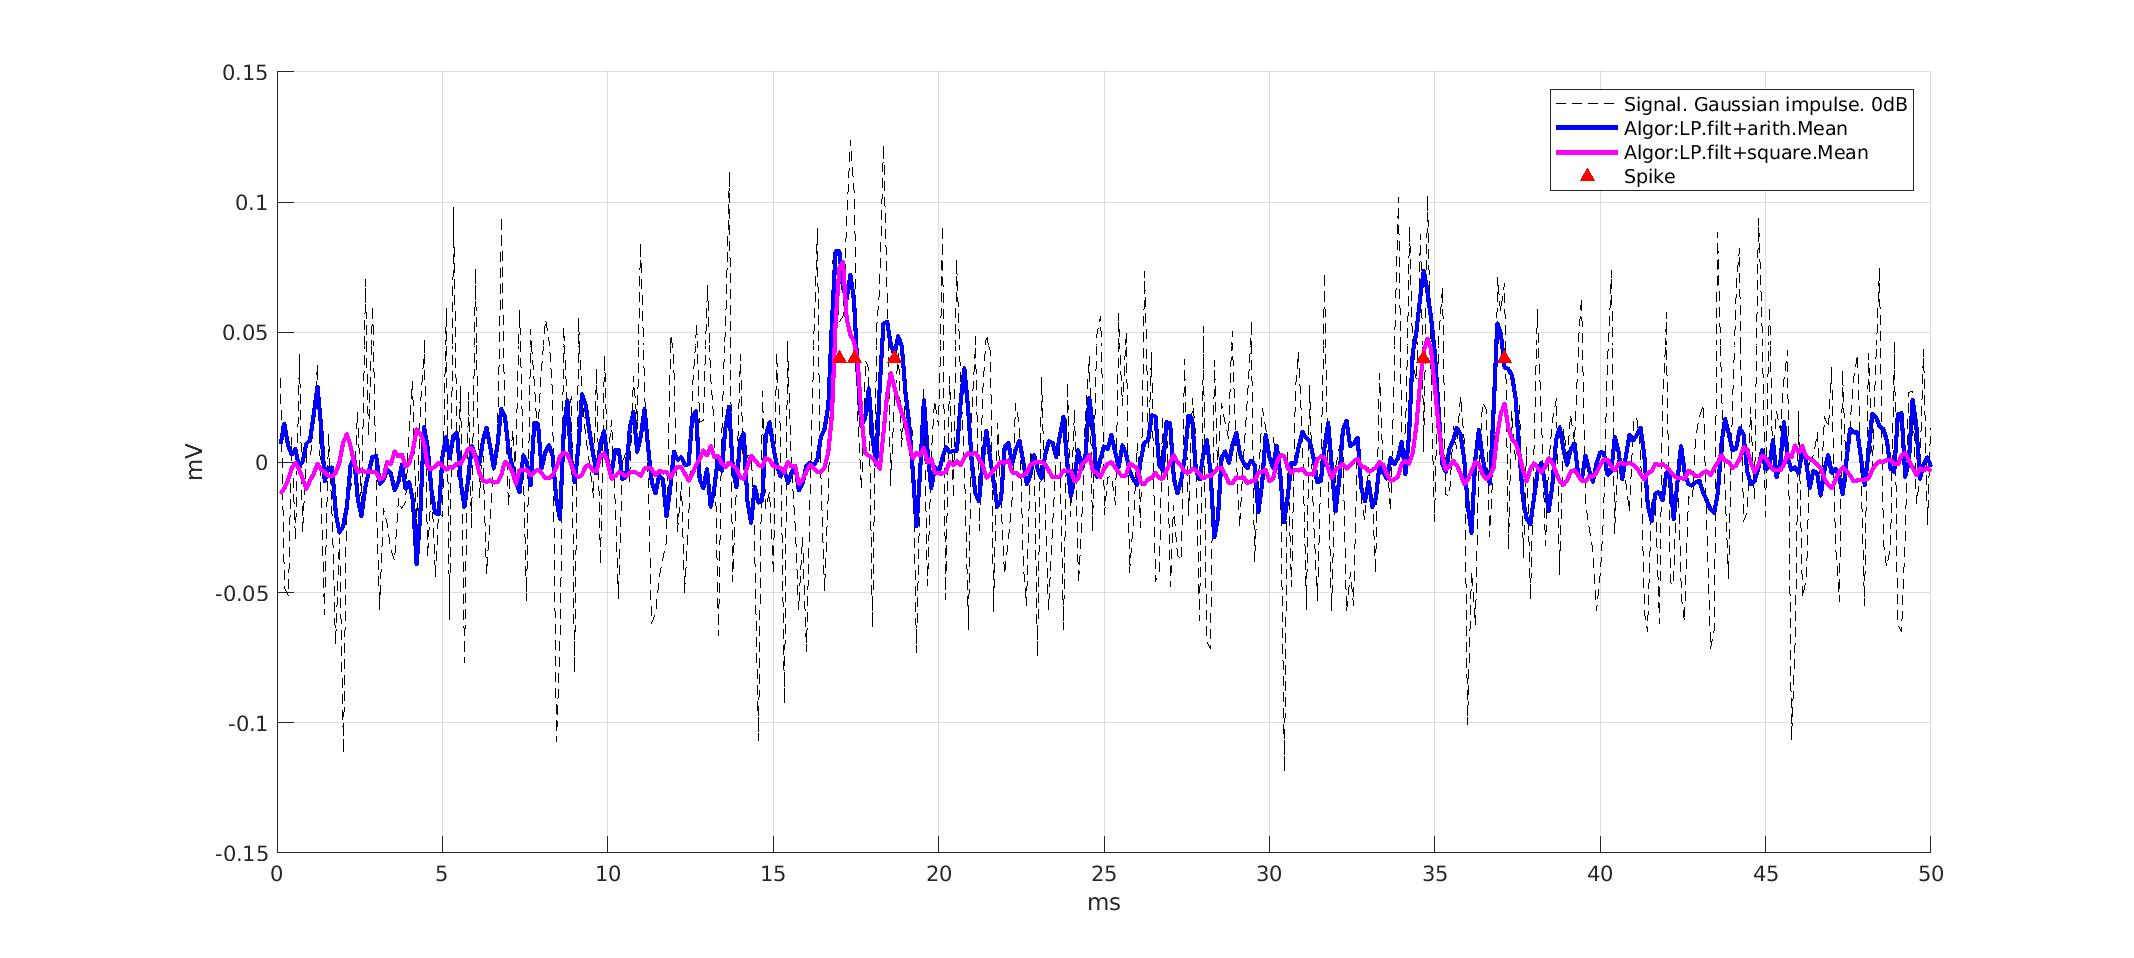
\includegraphics[width=1\linewidth]{results/c1_I2SNR0time.jpg}
\caption{Serie temporali. Segnale e filtri. Impulso gaussiano}
\label{fig:c1_I2SNR0time}
\end{figure}

\begin{figure}[htbp]
\centering
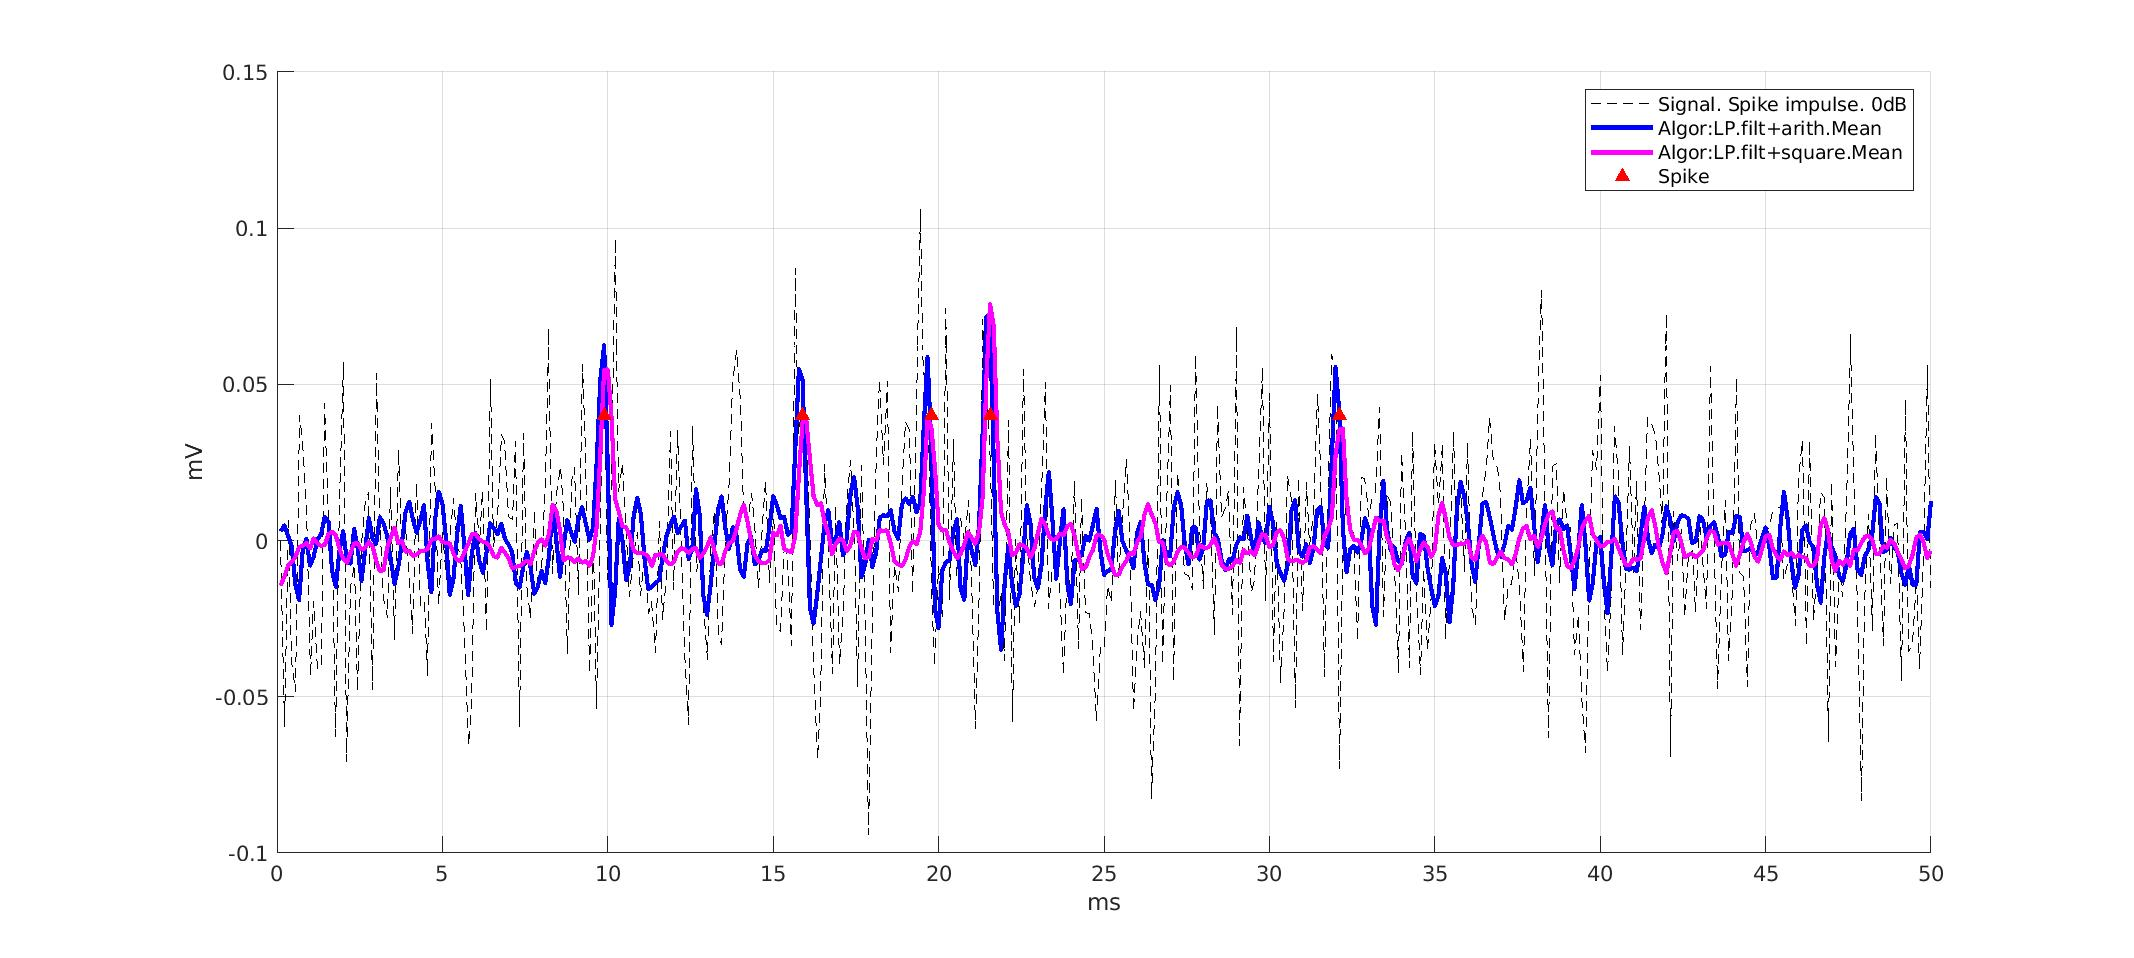
\includegraphics[width=1\linewidth]{results/c1_I4SNR0time.jpg}
\caption{Serie temporali. Segnale e filtri. Impulso spike}
\label{fig:c1_I4SNR0time}
\end{figure}




\section{Metriche di valutazione degli algoritmi}

Sotto il profilo spettrale, un buon filtro trasforma uno spettro rumoroso in modo da far emergere i picchi delle frequenza caratteristiche del segnale (toni) rispetto al rumore di fondo.
%
Nel contesto della presenza simulazione, dove il segnale è composto da impulsi di data forma funzionale, non necessariamente sinusoidale e di durata limitata, si deve tener conto anche di una visione {\it timbrica}, in cui rileva anche la forma caratteristica dei picchi e dello spettro in generale, forme che riflettono sia la forma funzionale degli impulsi sia le diverse irregolarità introdotte nel segnale.
%
In questo senso, un buon filtro dovrebbe restiture uno spettro del segnale rumoroso filtrato quanto più vicino a quello del segnale non rumoroso.
La metrica che valuta la distanza spettrale adottata in questo lavoro è presentata nel paragrafo \ref{metricaS}.

Sotto il profilo temporale invece, un buon algoritmo azzera il segnale dove non rileva impulsi in modo da ridurre gli errori di previsione di un test di soglia come il seguente
\begin{equation*}
t = t_{spike} \Leftrightarrow V(t) > V_{treshold}
\end{equation*}
Per test di soglia si intende perciò un criterio di discriminazione degli impulsi che si basa esclusivamente sull'ampiezza del segnale filtrato: scelto un valore di riferimento per il massimo rumore ammesso, tutti i punti del segnale sopra tale soglia si marcano come impulsi e come rumore il resto.
Tale procedura è chiaramente soggetta ad errore, la cui quantificazione 
attraverso opportune metriche da luogo alla valutazione di accuratezza dell'algoritmo adottato. In questo lavoro, la capacità predittiva degli algoritmi di sorting è valutata con la metrica illustrata nel paragrafo \ref{metricaT}.

Come illustrato nel paragrafo \ref{risultati}, le due metriche adottate sono fortemente correlate e l'analisi della loro congiunta distribuzione al variare del $SNR$ e della forma degli impulsi permette di valutarne la coerenza.



\subsection{Metriche: distanza spettrale}
\label{metricaS}

La distanza spettrale considerata è la distanza euclidea tra gli spettri nella banda $[0-\nu_{high}]$, dove $\nu_{high}$ è la frequenza alta di taglio del filtro passa banda.
% 
Nella formula che segue $DFT_{ref}$ è lo spettro del segnale di riferimento, non rumoroso e $DFT_{noisy.filt}$ quella del segnale rumoroso dopo essere stato soggetto agli algoritmi di sorting.
%
\begin{align*}
 d_{s}^2 & = \sum_{j:0}^{\nu_{high}}(DFT_{ref}(j) - DFT_{noisy.filt}(j) )^2
\end{align*}
%
L'indice $j$ corre solo nelle frequenze della banda di interesse, tenuto conto dei parametri di simulazione.




\subsection{Metriche: errore medio di previsione}
\label{metricaT}

Nel segnale di prova di riferimento sono noti i tempi di emissione degli impulsi.
%
Nel segnale filtrato questo tempo è incerto a causa dell'effetto congiunto della fase del filtro, della rumorosità del segnale e dell'azione dell'algoritmo.
%
La valutazione dell'errore medio di previsione è condotta con l'algoritmo \ref{alg:errore} nella seguente tabella.
%
\begin{algorithm}
\caption{Calcolo errore medio di previsione}\label{alg:errore}
\begin{algorithmic}[1]
%\Procedure{Euclid}{$a,b$}\Comment{The g.c.d. of a and b}
\State $t_{j=1,...,N}$ \Comment{Noti gli N tempi nel segnale di riferimento}
\State $\tau_{j=1,...,N}$ \Comment{Estraggo i primi N massimi nel segnale filtrato}
\State $\tau_{j}\mapsto d_{j} = min( |t_{1}-\tau_{j}|, |t_{2}-\tau_{j}|, ...)$ \Comment{Ad ogni previsione associo la minima distanza con l'insieme dei veri tempi $t_{j}$}
\State $\sum_{1}^{N} d_{j}/N$ \Comment{Errore medio in $ms$}
%\State $f_{t}\gets \sum_{i=1:3} f_{t-i}/3$
% \EndWhile\label{euclidendwhile}
% \State \textbf{return} $b$\Comment{The gcd is b}
% \EndProcedure
\end{algorithmic}
\end{algorithm}

Questa semplice metrica ha natura esplorativa ed è da intendersi solo indicativa della bontà di previsione, e viene utilizzata in questo lavoro solo per l'analisi esplorativa nei grafici di dispersione presentati qui di seguito. In particolare si evidenzia che la metrica non rileva in alcun modo la presenza di previsioni multiple sullo stesso impulso o la presenza di impulsi non rilevati.

Per completare l'analisi della capacità previsivia dei test, si utilizza invece un indicatore più formale. Qui di seguito illustrato nell'algoritmo \ref{alg:matrice}.

\begin{algorithm}
\caption{Calcolo errore medio di previsione}\label{alg:matrice}
\begin{algorithmic}[1]
%\Procedure{Euclid}{$a,b$}\Comment{The g.c.d. of a and b}
\State $t_{j=1,...,N}$ \Comment{Noti gli N tempi nel segnale di riferimento}
\State $\tau_{j=1,...,N}$ \Comment{Estraggo i primi N massimi nel segnale filtrato}
\State $\tau_{j}\mapsto d_{j} = min( |t_{1}-\tau_{j}|, |t_{2}-\tau_{j}|, ...)$ \Comment{Ad ogni previsione associo la minima distanza con l'insieme dei veri tempi $t_{j}$}
\State Se $d_{j}<\frac{D}{2}$ \Comment{Se l'errore è minore della semidurata degli impulsi allora la previsione si intende corretta. L'impulso viene marcato come rilevato, se già non lo era da una precedente previsione.}
\State Se $d_{j}>\frac{D}{2}$ \Comment{Se l'errore è maggiore della semidurata degli impulsi allora la previsione si intende errata. L'evento viene marcato come un falso positivo, se già non lo era da una precedente previsione.}
\State  \Comment{Il numero di falsi negativi si determina per differenza di $N$ con gli impulsi rilevati.}
\State  \Comment{Il numero di veri negativi si determina per differenza di $N$ con il numero di falsi positivi.}
\end{algorithmic}
\end{algorithm}

In breve, data una media di $150$ impulsi in un segnale della durata di $1s$, l'algoritmo registra gli impulsi rilevati e determina quelli non rilevati per differenza. La registrazione è dicotomica, non si contano cioè il numero di previsioni che rilevano lo stesso impulso. Simmetricamente, il segnale può essere scomposto in $150$ spazi vuoti che rappresentano i tempi di attesa tra due impulsi. L'algoritmo conta gli spazi vuoti che ricevono una previsione di impulso e determina così i falsi positivi e, per differenza, i veri negativi.

L'applicazione di questo algoritmo riassume tutta la simulazione in una matrice $2x2$ che rappresenta la distribuzione congiunta dei tempi di emissione previsti e di quelli effettivi. Maggiori sono gli elementi concordanti della matrice, quelli cioè posti sulla diagonale principale, dove a impulsi effettivi corrispondono impulsi previsti e viceversa, maggiore sarà la bontà dell'algoritmo.

Si osserva che nell'applicazione di questo algoritmo è implicita una tolleranza nella previsione del tempo d'impulso pari alla durata dell'impulso stesso.

Infine, dati i parametri di simulazione utilizzati, la lunghezza di un impulso che è di $9$ campioni e la distanza media tra gli impulsi di $60$ campioni, un algoritmo casuale di rilevazione ha una matrice degli errori caratteristica basata sul {\it fattore casuale di successo} di $\frac{9}{60}$ di cui bisogna tener conto in sede di valutazione dei risultati. 



\section{Risultati}
\label{risultati}

I grafici \ref{fig:scatter1} $-$ \ref{fig:scatter5} mostrano la distribuzione congiunta delle metriche temporale e spettrale. Come atteso, si evidenzia (1) una forte correlazione positiva tra le due metriche, (2) l'andamento crescente con il decrescere del $SNR$, (3) una distinta collazione dei punti in base all'algoritmo di sorting e al tipo di impulso.

Per quanto riguarda gli impulsi rettangolare e gaussiano si evidenziano due fasi. La prima con $SNR$ fino a $-12$ $dB$, l'errore medio di previsione mostra un andamento simile per le due categorie di test, quadratico e semplice, se non addirittura favorevole al test quadratico. Poi per $SNR$ inferiori, si evidenzia una marcata divergenza delle performance dei test a media quadratica, come se l'aumento della rumorosità avesse l'effetto congiunto di distorcere lo spettro e peggiorare la precisione con cui si determinano i momenti degli impulsi. L'andamento delle due metriche è concorde, come previsto. Per quanto riguarda l'impulso sinusoidale si evidenzia invece una netta separazione nelle performance previsive dei due algoritmi.

Tuttavia ciò che indebolisce l'evidenza riportata da questi grafici è il valore medio della distanza temporale, mai superiore a $1$ $ms$; sebbene l'andamento sia peggiorativo con l'$SNR$, l'errore di previsione medio non è mai superiore alla semidurata degli impulsi. Tale considerazione fa sospettare che le {\it differenze visive di natura grafica} siano dovute esclusivamente alla differenza di rilevazione del centro dell'impulso, indotte dalla diversa forma funzionale. In particolare, impulsi simmetrici (gaussiano, rettangolare) vengono meglio rilevati rispetto a quelli asimmetrici (sinusoidale, neurale). Risulta a questo punto necessaria un'analisi più approfondita.


\begin{figure}[htbp]
\centering
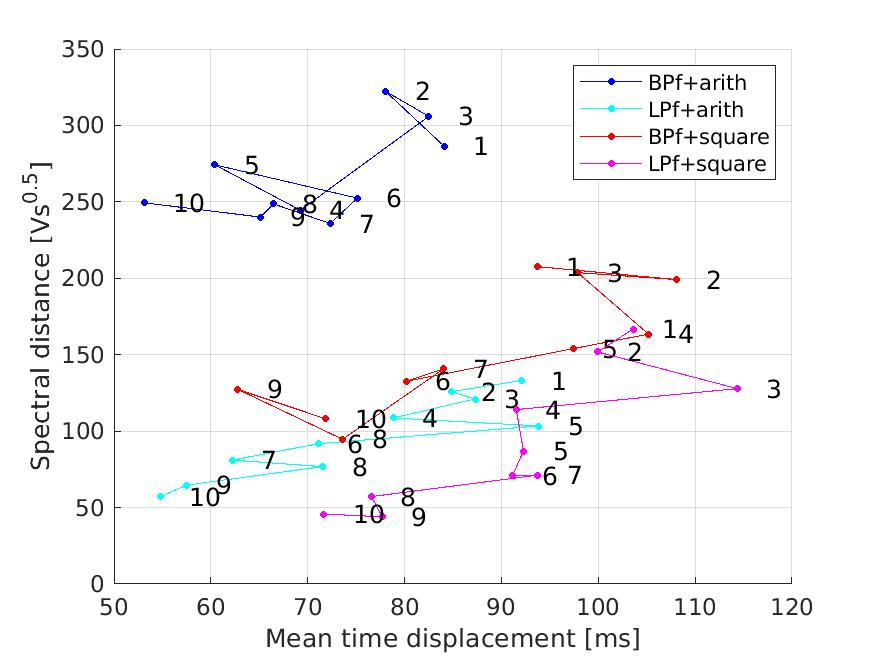
\includegraphics[width=1\linewidth]{graphs/scatter1.jpg}
\caption{Impulso rettangolare. $SNR= \{-12,-3\}dB$}
\label{fig:scatter1}
\end{figure}

\begin{figure}[htbp]
\centering
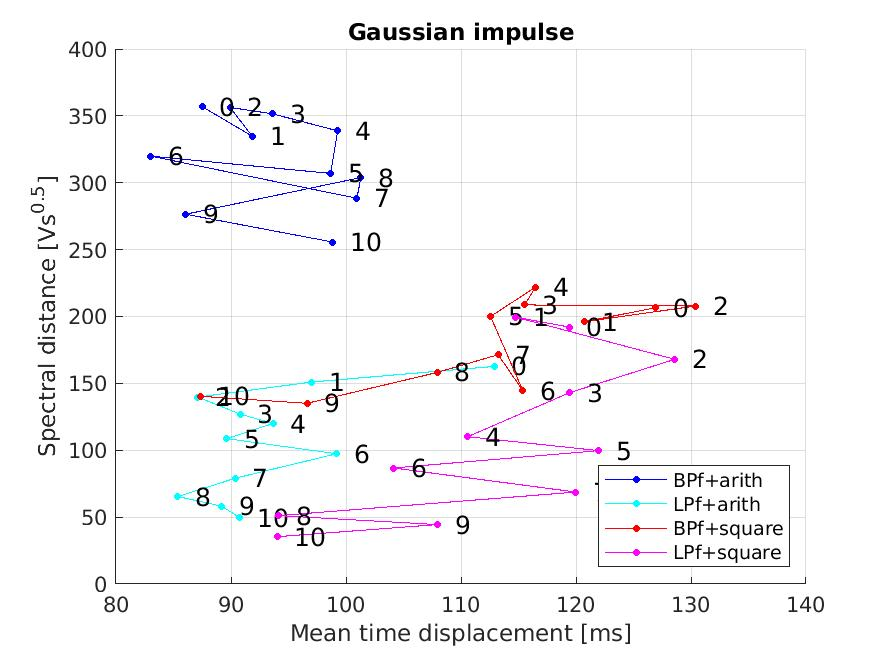
\includegraphics[width=1\linewidth]{graphs/scatter2.jpg}
\caption{Impulso gaussiano. $SNR= \{-12,-3\}dB$}
\label{fig:scatter2}
\end{figure}

\begin{figure}[htbp]
\centering
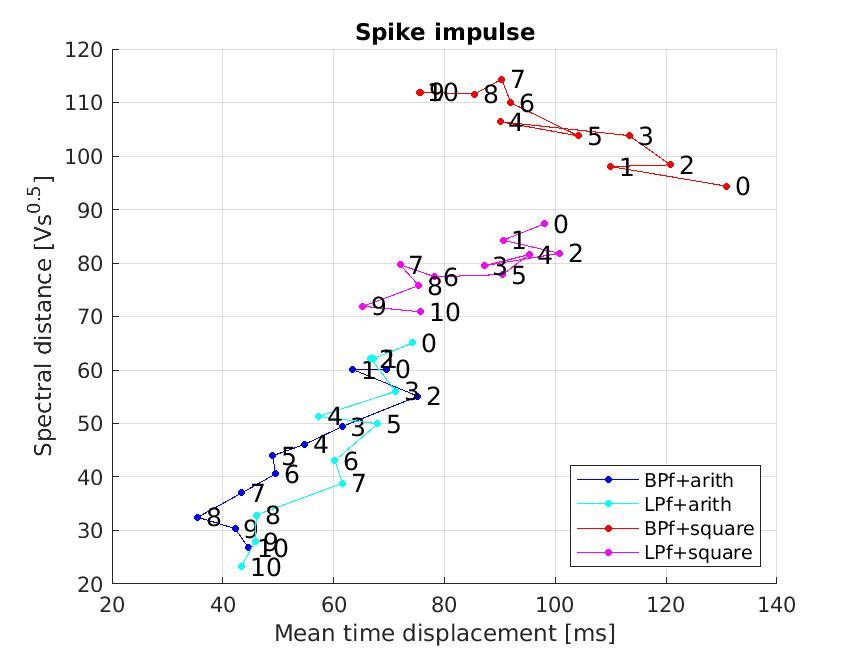
\includegraphics[width=1\linewidth]{graphs/scatter4.jpg}
\caption{Impulso neurale. $SNR= \{-12,-3\}dB$}
\label{fig:scatter4}
\end{figure}

\begin{figure}[htbp]
\centering
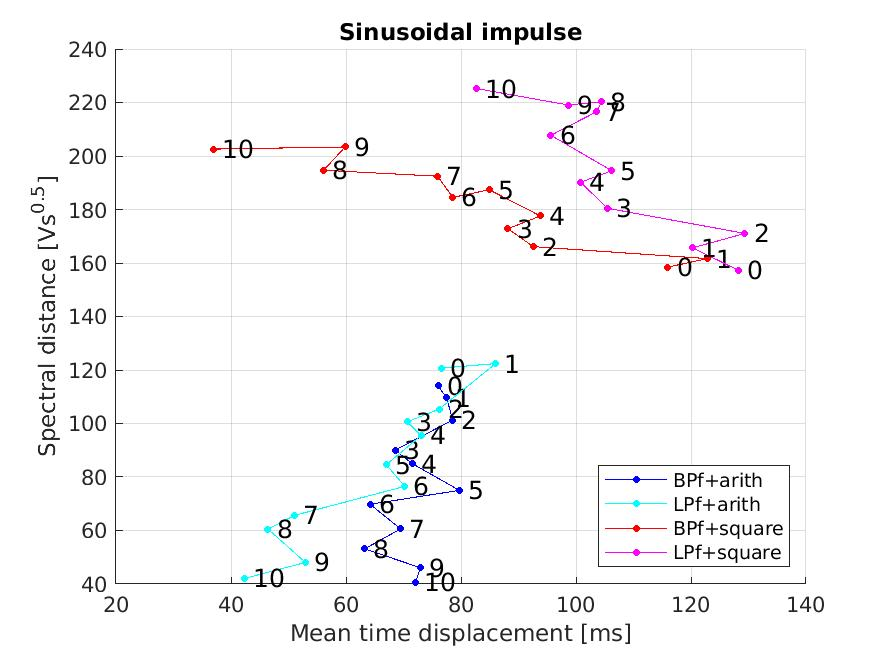
\includegraphics[width=1\linewidth]{graphs/scatter5.jpg}
\caption{Impulso sinusoidale. $SNR= \{-12,-3\}dB$}
\label{fig:scatter5}
\end{figure}



%-----------------------------------------
%-----------------------------------------
%-----------------------------------------
\section{Accuratezza}
\label{accuratezza}


\subsection{Indici di accuratezza}
\label{indici}
Nella tabella \ref{tab:indici} i filtri preliminari in frequenza sono indicati con
$BP$: passa banda,
$LP$: passa basso.
I test invece con
$1$: semplice, a media aritmetica, il test di riferimento.
$2$: quadratico, il test in potenza in valutazione.

Il valore numerico degli indici in tabella evidenzia la superiorità dei test in tensione a media semplice, con indici di concorcadanza medi sempre superiori ai test a media quadratica.

\begin{table}[htbp]
\centering
\caption{\bf Accuratezza}
\begin{tabular}{ccccc}
\hline
%Test              & \multirow{2}{}{Semplice} & \multirow{2}{}{Quadratico} \\
Test                & BP-1 & BP-2 & LP-1 & LP-2 \\
\hline
Punteggio F1        & 0.3384    &0.2159    &0.3349    &0.2211\\
Indice di Jaccard   & 0.7336    &0.5795    &0.7281    &0.5886 \\
\hline
\end{tabular}
\label{tab:indici}
\end{table}


\subsection{Matrici di accuratezza}
\label{matrici}

Il dettaglio delle matrici di accuratezza da cui sono stati calcolati gli indici al paragrafo \ref{indici} è qui di seguito riportato.

%
\begin{table}[htbp]
\centering
\begin{tabular}{cccclcc}
                           &                         & \multicolumn{2}{c}{BP-1}                           &                       & \multicolumn{2}{c}{BP-2}                           \\
                           &                         & \multicolumn{2}{c}{Previsto}                       &                       & \multicolumn{2}{c}{Previsto}                       \\
                           &                         & si                      & no                       &                       & si                      & no                       \\ \cline{3-4} \cline{6-7} 
\multirow{2}{*}{Effettivo} & \multicolumn{1}{c|}{si} & \multicolumn{1}{c|}{83} & \multicolumn{1}{c|}{67} & \multicolumn{1}{l|}{} & \multicolumn{1}{c|}{48} & \multicolumn{1}{c|}{102} \\ \cline{3-4} \cline{6-7} 
                           & \multicolumn{1}{c|}{no} & \multicolumn{1}{c|}{13} & \multicolumn{1}{c|}{137} & \multicolumn{1}{l|}{} & \multicolumn{1}{c|}{24} & \multicolumn{1}{c|}{126} \\ \cline{3-4} \cline{6-7} 
                           &                         &                         &                          &                       &                         &                          \\
                           &                         & \multicolumn{2}{c}{LP-1}                           &                       & \multicolumn{2}{c}{LP-2}                           \\
                           &                         & \multicolumn{2}{c}{Previsto}                       &                       & \multicolumn{2}{c}{Previsto}                       \\
                           &                         & si                      & no                       &                       & si                      & no                       \\ \cline{3-4} \cline{6-7} 
Effettivo                  & \multicolumn{1}{c|}{si} & \multicolumn{1}{c|}{82} & \multicolumn{1}{c|}{68} & \multicolumn{1}{l|}{} & \multicolumn{1}{c|}{49} & \multicolumn{1}{c|}{101} \\ \cline{3-4} \cline{6-7} 
                           & \multicolumn{1}{c|}{no} & \multicolumn{1}{c|}{14} & \multicolumn{1}{c|}{136} & \multicolumn{1}{l|}{} & \multicolumn{1}{c|}{22} & \multicolumn{1}{c|}{128} \\ \cline{3-4} \cline{6-7} 
\end{tabular}
\caption{\bf Accuratezza}
\label{tab:matrici}
\end{table}
%



%-----------------------------------------
%-----------------------------------------
%-----------------------------------------
\section{Conclusioni}
\label{conclusioni}

In tutti i casi considerati, al variare del $SNR$ e della forma dell'impulso, il test che garantisce miglior capacità previsiva è quello a media semplice.

\subsection{Filtro LP vs BP}
Dai risultati riportati si evidenzia scarsa rilevanza del tipo di filtro applicato. Come da attese infatti, il picco in frequenza relativo allo {\it spike rate} è lontano dalle soglie di banda dei filtri utilizzati e nel segnale simulato non sono state introdotte oscillazioni di bassa frequenza, unica circostanza che giustificherebbe l'applicazione del filtro passa alto.


\subsection{Media semplice vs quadratica}
A priori, sono diverse le considerazioni che si possono muovere a sfavore dell'efficacia degli algoritmi di sorting in potenza a media quadratica in un contesto di alta rumorosità e irregolarità del segnale. In primo luogo, l'applicazione del quadrato non permette di sfruttare l'elevata frequenza di campionamento spazio temporale per mediare segnali da pixel diversi e ridurre così compensativamente il rumore. In secondo luogo, laddove gli impulsi sono irregolari e limitati nel tempo l'applicazione di una trasformazione non lineare ad un pacchetto di frequenze comporta distorsioni allo spettro facendo comparire, in seguito all'elevamente al quadrato, picchi spettrali che non sono invece presenti nel segnale originale. D'altro canto, i test a media semplice non inducono alcuna distorsione spettrale e permettono di mediare il rumore tra diversi pixel. A sfavore dei test in tensione a media semplice, si può invece argomentare che in presenza di impulsi a media nulla, con parti positive e negative, una delle due non può essere utilizzata per rilevare gli impulsi con test di soglia.
%
I risultati qui esposti dimostrano che le distorsioni spettrali introdotte dai test a media quadratica, il comparire cioè di picchi in frequenza non presenti nello spettro originale a causa dell'elevamento al quadrato, sebbene non risultino visibili graficamente, in quanto smorzati dall'irregolarità del segnale, sono comunque rilevati dalla metrica di distanza spettrale e contribuiscono a deteriorare la capacità previsiva di questa categoria di test.
%
I test a media semplice, per contro, risultano molto precisi sia nella sagoma spettrale restituita, sia nella rilevazione del tempo degli impulsi. Inoltre, l'insieme degli impulsi correttamente rilevati da questi test è maggiore rispetto a quello dei test a media quadratica, come evidenziato dai conteggi riportati nelle matrici di errore.
%
Le risultanze intermedie dei grafici di andamento congiunto vengono periò confermate. Sebbene le differenze grafiche visive siano da attribuire a differenze nella rilevazione del centro dell'impulso, in funzione delle diverse forme funzionali degli impulsi utilizzati, l'andamento crescente dell'errore di previsione è effettivamente indicativo del deterioramento delle capacità previsive dei test a media quadratica, sebbene i valori di errore medio siano molto bassi. Circostanza che si spiega per l'elevata percentuale di impulsi correttamente previsti, che abbassa i valori dell'errore medio di entrambe le categorie di test.


\section{Riferimenti bibliografici}

% Full references (to aid the editor and reviewers) must be included. This will be produced automatically if you are using a .bib file.

% \bigskip
% \noindent Add citations manually or use BibTeX. See \cite{Chitimalla:17,Wen:16}.

% Bibliography
\bibliography{biblio/biblio.bib}

%Manual citation list
%\begin{thebibliography}{1}
%\bibitem{Zhang:14}
%Y.~Zhang, S.~Qiao, L.~Sun, Q.~W. Shi, W.~Huang, %L.~Li, and Z.~Yang,
 % \enquote{Photoinduced active terahertz metamaterials with nanostructured
  %vanadium dioxide film deposited by sol-gel method,} Opt. Express \textbf{22},
  %11070--11078 (2014).
%\end{thebibliography}




% JOCN authors may include their biographies and photos. This section is not required 

% \section*{Author Biographies}
% 
% \setlength\intextsep{0pt}
% 

% \paragraph{}
% \noindent \textbf{First A. Author} (M’76–SM’81–F’87) and the other authors may include biographies at the end of regular papers. This author became a Member (M) of IEEE in 1976, a Senior Member (SM) in 1981, and a Fellow (F) in 1987. The first paragraph may contain a place and/or date of birth (list place, then date). Next, the author’s educational background is listed. The degrees should be listed with type of degree in what field, which institution, city, state, and country, and year degree was earned. The author’s major field of study should be lower-cased.
  


% \begin{wrapfigure}{L}{0.21\textwidth}
%      \includegraphics[width=0.2\textwidth]{alicesmith}
%    \end{wrapfigure}
%    \noindent
%    \textbf{Alice Smith} received her BSc (Mathematics) in 2000 from The University of Maryland. Her research interests also include lasers and optics.\\
  
  

  
\pagebreak

% \section{Appendix}
% 
% 
% \subsection{Densità spettrali}
% 
% 
% \begin{figure}[htbp]
% \centering
% \fbox{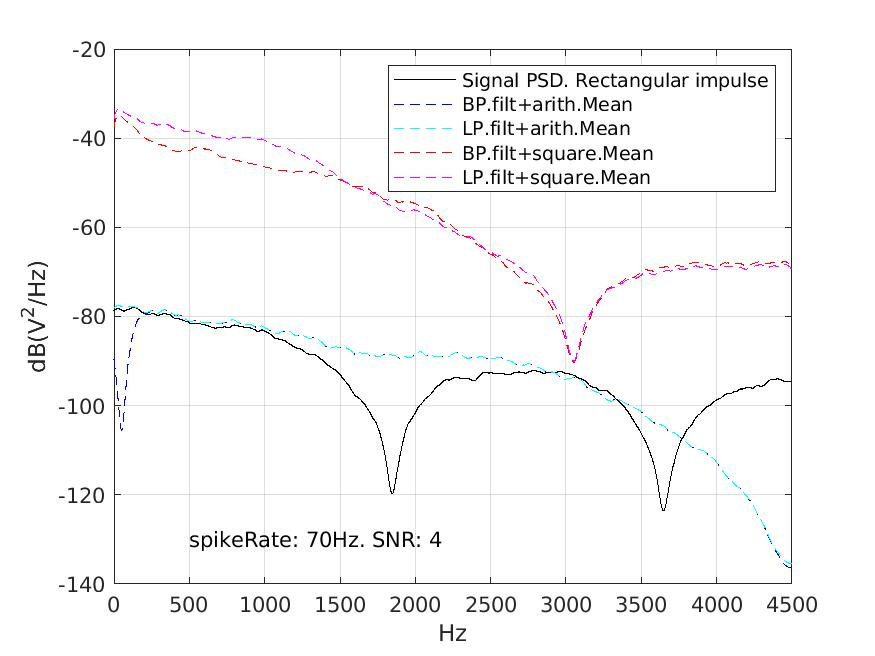
\includegraphics[width=1\linewidth]{results/c9_I1SNR4spec.jpg}}
% \caption{Spectral density of signal and filtered signal.}
% \label{fig:c9_I1SNR4spec}
% \end{figure}
% 
% \begin{figure}[htbp]
% \centering
% \fbox{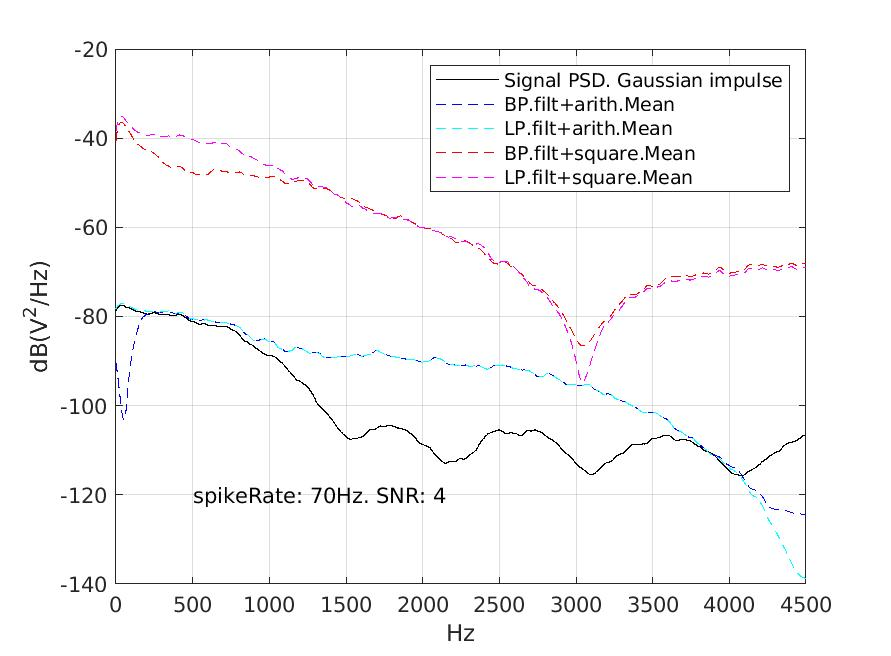
\includegraphics[width=1\linewidth]{results/c9_I2SNR4spec.jpg}}
% \caption{Spectral density of signal and filtered signal.}
% \label{fig:c9_I2SNR4spec}
% \end{figure}
% 
% \begin{figure}[htbp]
% \centering
% \fbox{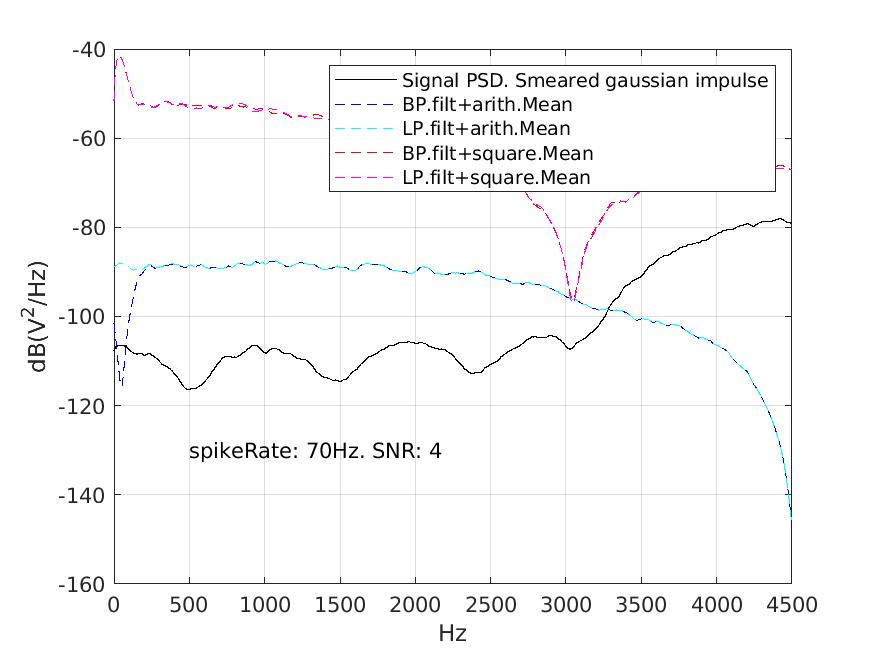
\includegraphics[width=1\linewidth]{results/c9_I3SNR4spec.jpg}}
% \caption{Spectral density of signal and filtered signal.}
% \label{fig:c9_I3SNR4spec}
% \end{figure}
% 
% \begin{figure}[htbp]
% \centering
% \fbox{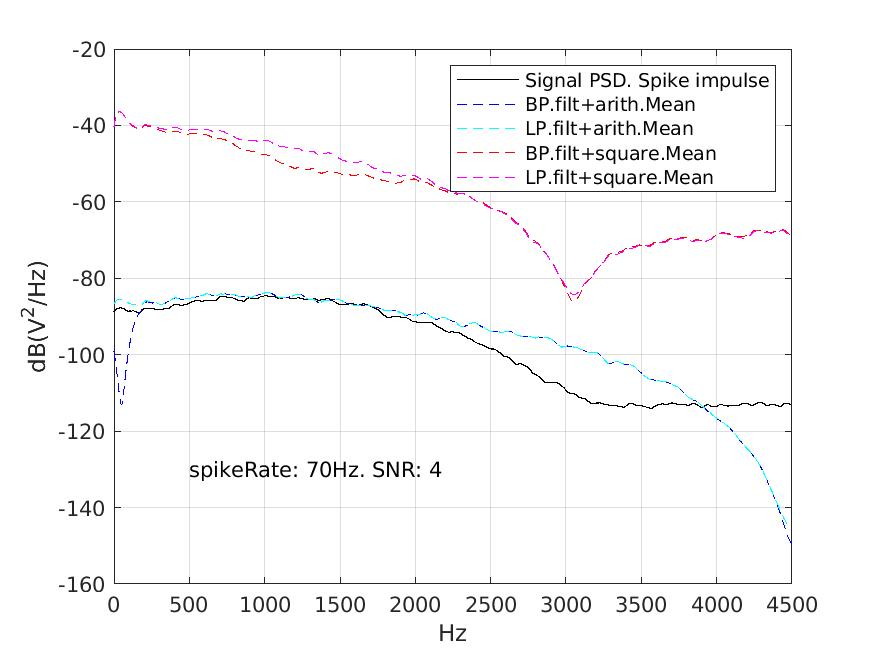
\includegraphics[width=1\linewidth]{results/c9_I4SNR4spec.jpg}}
% \caption{Spectral density of signal and filtered signal.}
% \label{fig:c9_I4SNR4spec}
% \end{figure}
% 
% \begin{figure}[htbp]
% \centering
% \fbox{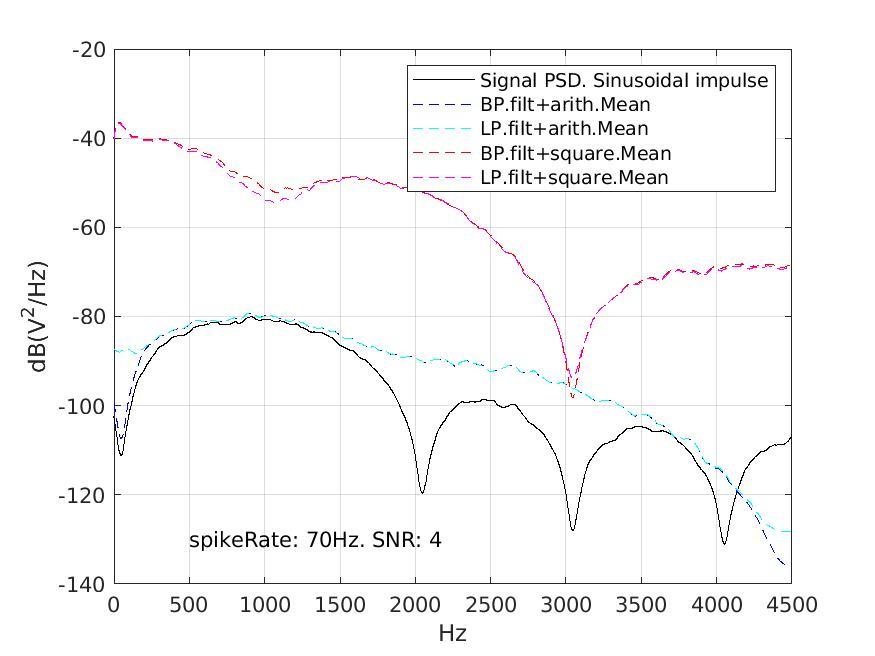
\includegraphics[width=1\linewidth]{results/c9_I5SNR4spec.jpg}}
% \caption{Spectral density of signal and filtered signal.}
% \label{fig:c9_I5SNR4spec}
% \end{figure}
% 
% 
% 
% \subsection{Distribuzione congiunta metriche}
% 
% 
% \begin{figure}[htbp]
% \centering
% \fbox{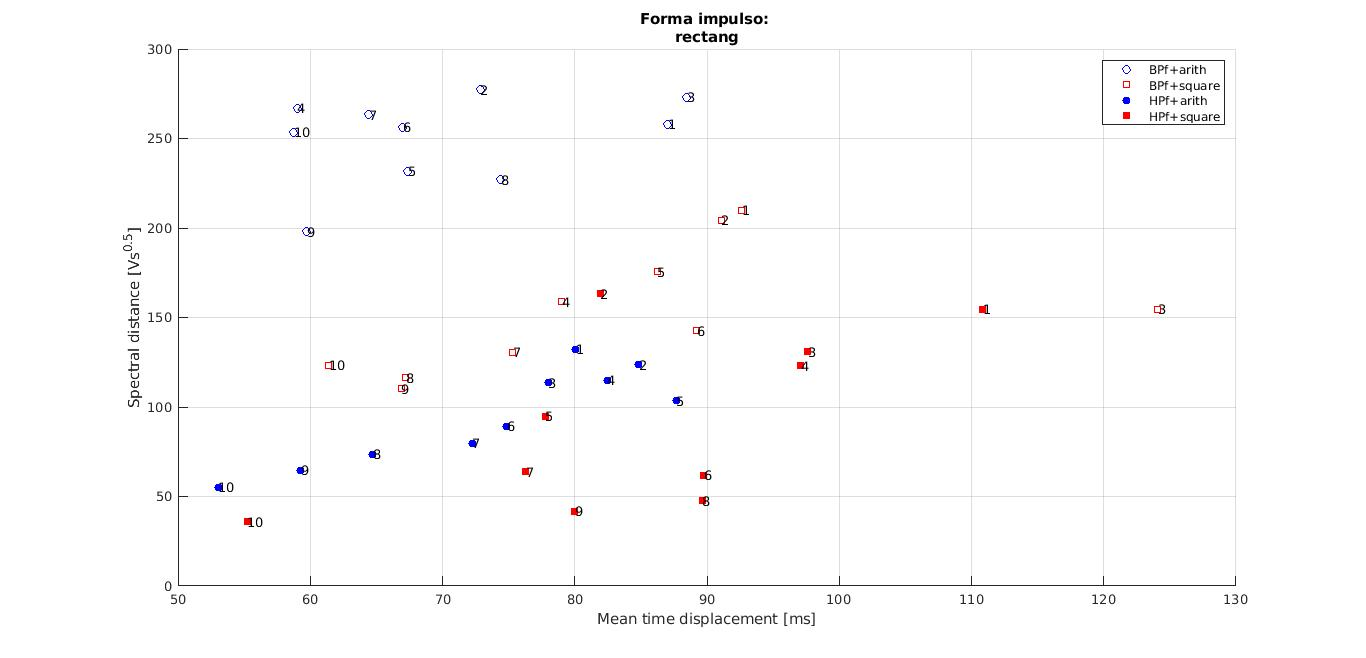
\includegraphics[width=.8\linewidth]{results/rectaScatter.jpg}}
% \caption{Impulso rettangolare. Metriche di valutazione.}
% \label{fig:rectaScatter}
% \end{figure}
% 
% \begin{figure}[htbp]
% \centering
% \fbox{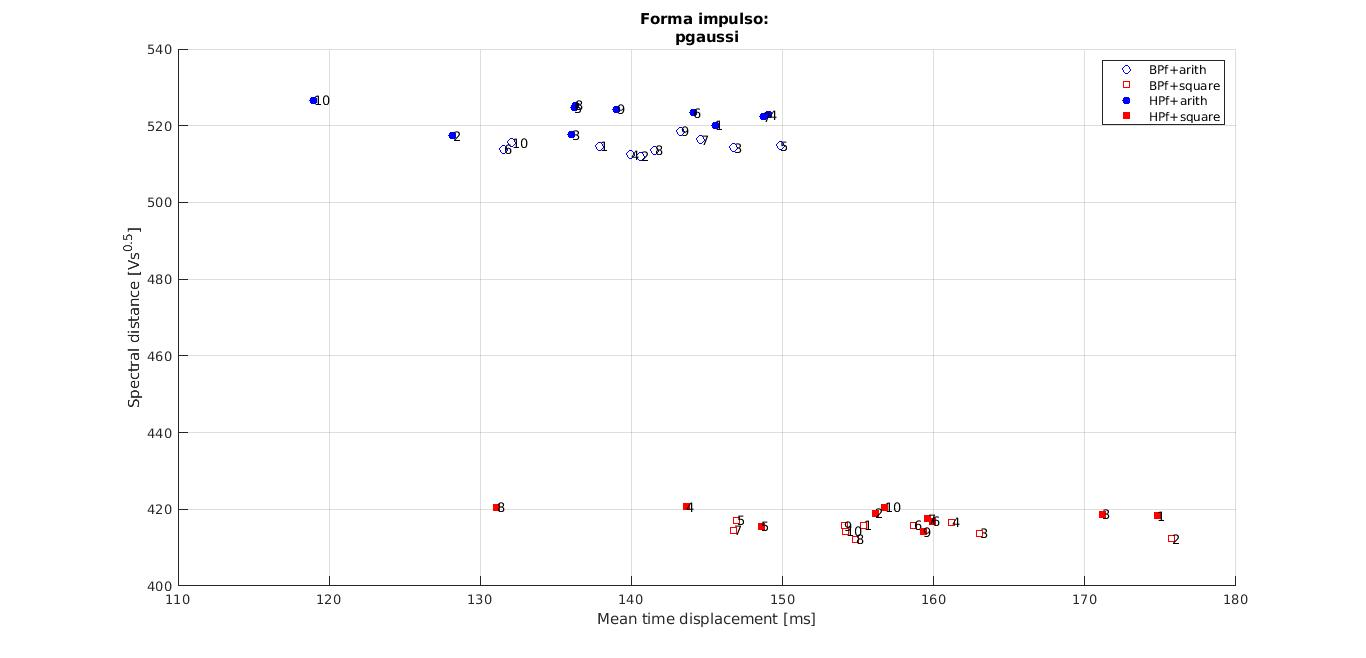
\includegraphics[width=.8\linewidth]{results/pgaussScatter.jpg}}
% \caption{Impulso gaussiano sfasato. Metriche di valutazione.}
% \label{fig:pgaussScatter}
% \end{figure}
% 
% \begin{figure}[htbp]
% \centering
% \fbox{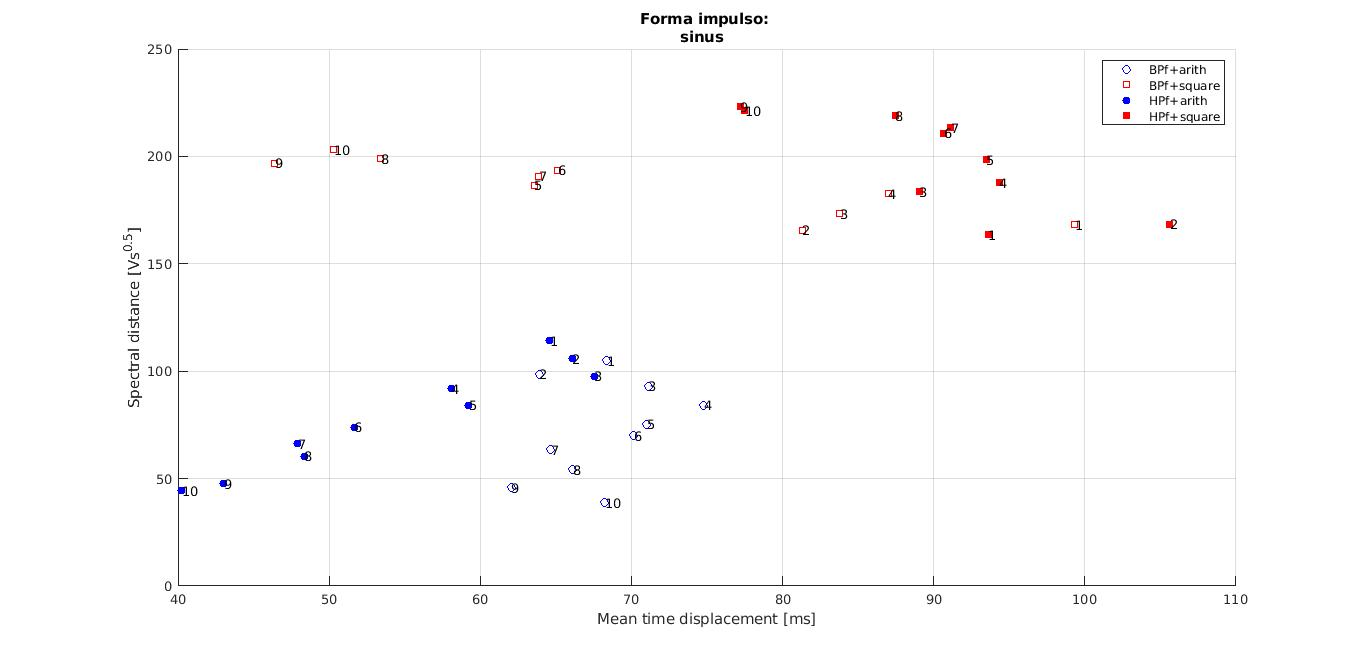
\includegraphics[width=.8\linewidth]{results/sinusScatter.jpg}}
% \caption{Impulso sinusoidale. Metriche di valutazione.}
% \label{fig:sinusScatter}
% \end{figure}


\end{document}




% \begin{algorithm}
% \caption{Euclid’s algorithm}\label{alg:euclid}
% \begin{algorithmic}[1]
% \Procedure{Euclid}{$a,b$}\Comment{The g.c.d. of a and b}
% \State $r\gets a\bmod b$
% \While{$r\not=0$}\Comment{We have the answer if r is 0}
% \State $a\gets b$
% \State $b\gets r$
% \State $r\gets a\bmod b$
% \EndWhile\label{euclidendwhile}
% \State \textbf{return} $b$\Comment{The gcd is b}
% \EndProcedure
% \end{algorithmic}
% \end{algorithm}
